%\vspace{1.5\baselineskip}
\begin{figure}[H]
    \begin{center}
    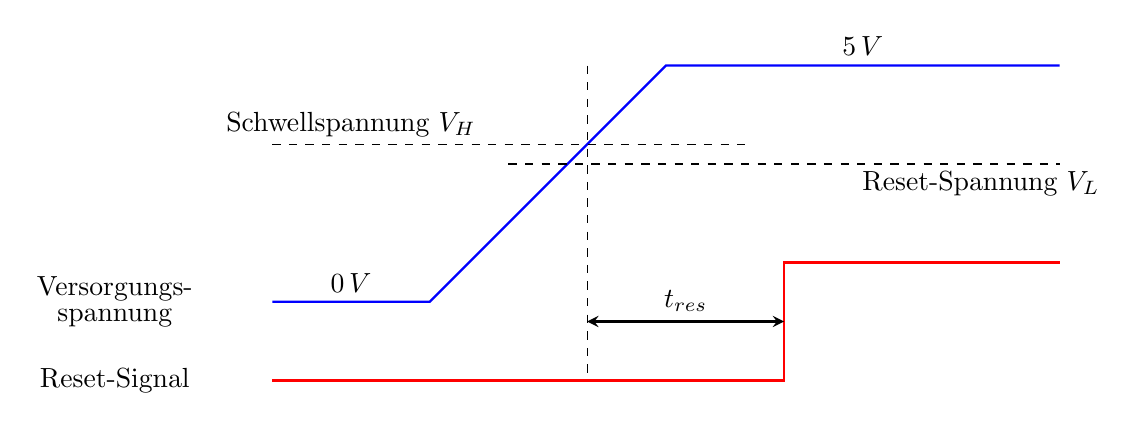
\begin{tikzpicture}
        % Achsen
        % \draw[->] (0,0) -- (10,0) node[anchor=north] {s}; % x-Achse
        % \draw[->] (0,0) -- (0,4) node[anchor=east] {V}; % y-Achse

        % Linie
        \draw[thick, blue] 
            (0,0) -- (2,0) % waagerechter Teil von 0 bis 2 Sekunden
            to (5,3) -- ++(5,0);
            % Kreuzungspunkt berechnen
        \coordinate (Kreuzung) at (4,2);

        
        \draw[thick, red] 
            (0,-1) -- ++(6.5,0) -- ++(0,1.5) -- ++(3.5,0);

        % Gestrichelte Linien
        \draw[dashed] 
            (0,2) -- ++ (6,0); % Senkrechte Linie nach unten
        \draw[dashed] 
            (4,3) -- ++(0,-4); % Waagerechte Linie nach rechts
        \draw[dashed] 
            (3,1.75) -- ++(7,0);
            
        % Beschriftungen
        \node[anchor=south, xshift=1cm] at (0,0) {$0\,V$}; % Startpunktbeschriftung
        \node[anchor=south] at (7.5,3) {$5\,V$}; % Endpunktbeschriftung
        \node[] at (-2,0) {\shortstack{Versorgungs- \\spannung}};
        \node[] at (-2,-1) {\shortstack{Reset-Signal}};
        \node[] at (1,2.25) {\shortstack{Schwellspannung $V_H$}};
        \node[] at (9,1.5) {\shortstack{Reset-Spannung $V_L$}};


        \draw[<->, thick, >=stealth] (4,-0.25) -- ++(2.5,0) node[midway, above] {$t_{res}$}; % Pfeil

        
    \end{tikzpicture}        

    \end{center}
    \caption[Schwellspannung]{\\Quelle: Schwellspannung (Eigene Darstellung)}
    \label{fig:Schwellspannung}
\end{figure}
%\vspace{1.5\baselineskip}